\newpage
\section{Question 3}
	\subsection*{The Iterated Closed Loop Algorithm}
	\noindent
	\newline
	By modifying the given code pieces, we will implement an Iterated Closed Loop algorithm to estimate the position of a vehicle as it moves through its surroundings.\newline All code pieces, original and modified, can be found in Appendix A [3].
		\subsubsection{Part A - Implementing the ICP}
		\newline
		By modifying the given showICP.m file, we will exam the resultant ICP features generated for a single data set. The set in question is frame 500, and we will use frame 520 as our initial 'guess'.\newline Firstly, using the default variables of a grid size of 0.005, and a maximum iterative loop of 40, we can generate the following graph:\newline
			\begin{figure}[position = here]
				\begin{centering}
					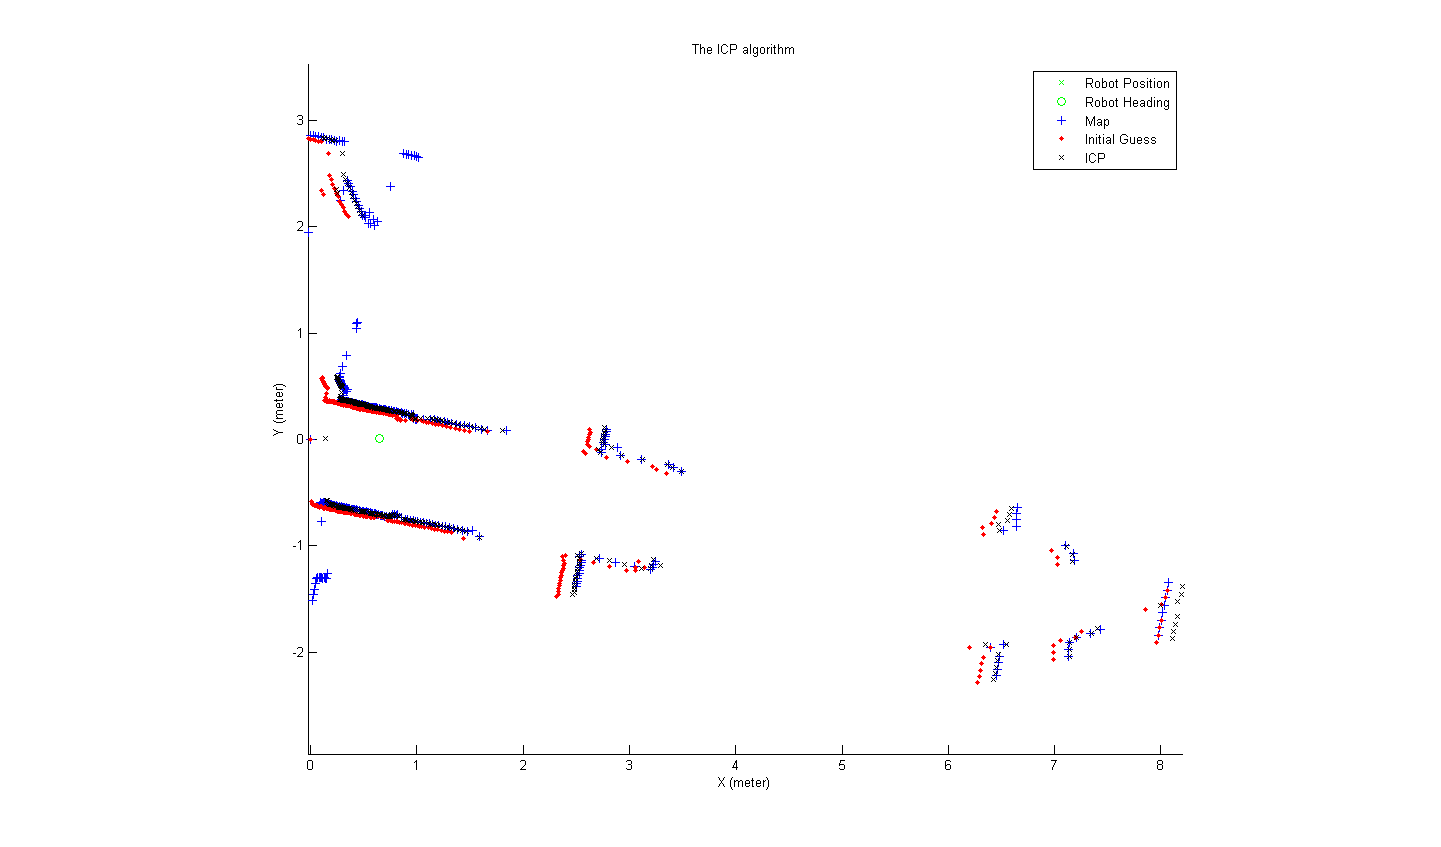
\includegraphics[scale=0.5]{q3a_1_1}\\
					\caption[\textit{RPYAxes}]{ICP estimate for maximum iterations of 40 and grid size of 0.005}
				\end{centering}
			\end{figure}
		\newline
		We will now examine the effect of modifying some of the variables of the ICPv4.m algorithm.\newline Firstly we will look at changing the grid size. For a smaller grid size of 0.001 we obtain the following graph:\newline
		
			\begin{figure}[position = here]
				\begin{centering}
					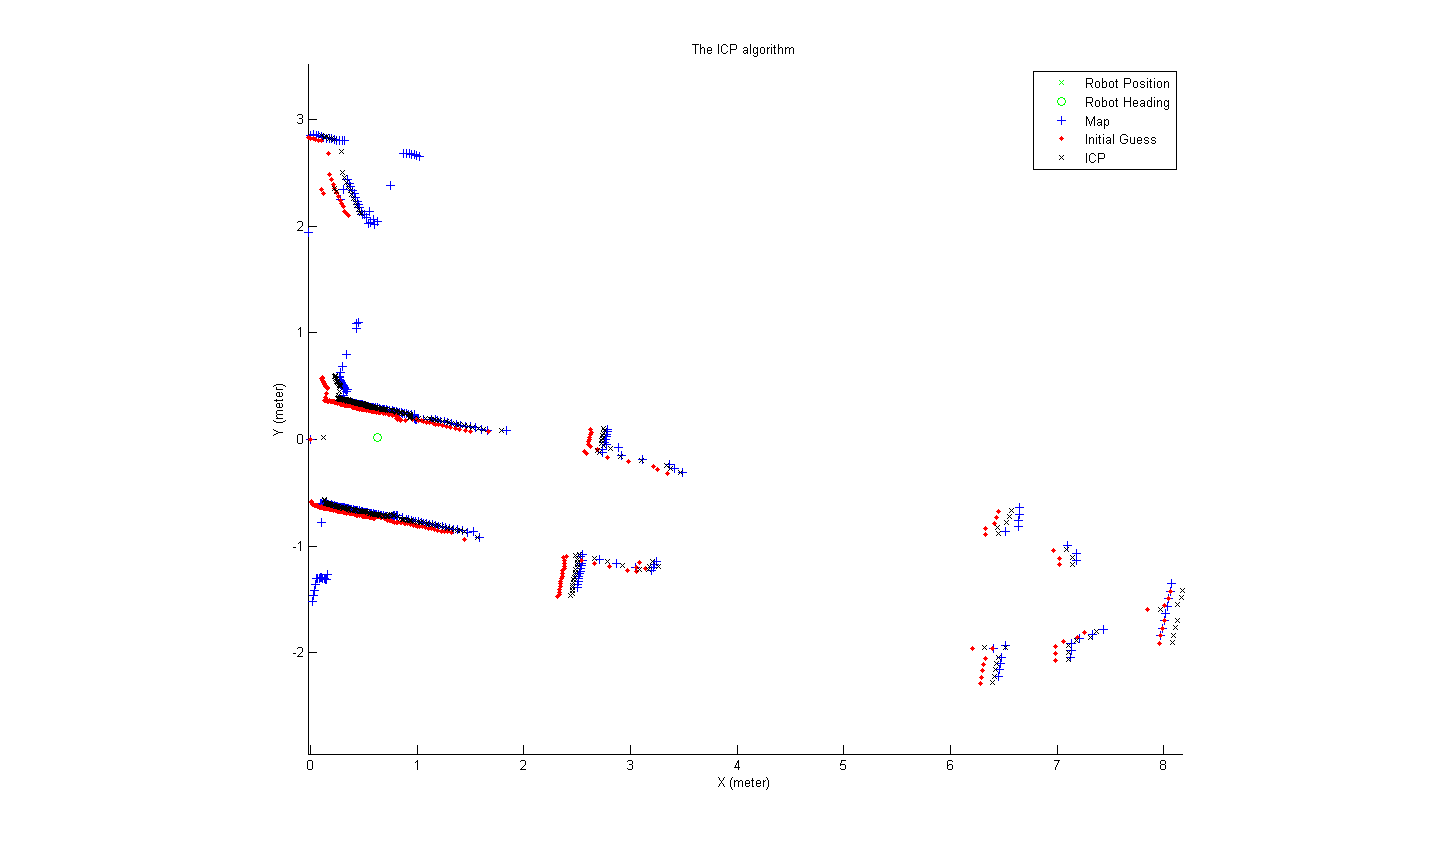
\includegraphics[scale=0.5]{q3a_1_2}\\
					\caption[\textit{RPYAxes}]{ICP estimate for maximum iterations of 40 and grid size of 0.001}
				\end{centering}
			\end{figure}
			
		\newline	
		\pagebreak	
		Next, for a grid size of 0.1:\newline
		
			\begin{figure}[position = here]
				\begin{centering}
					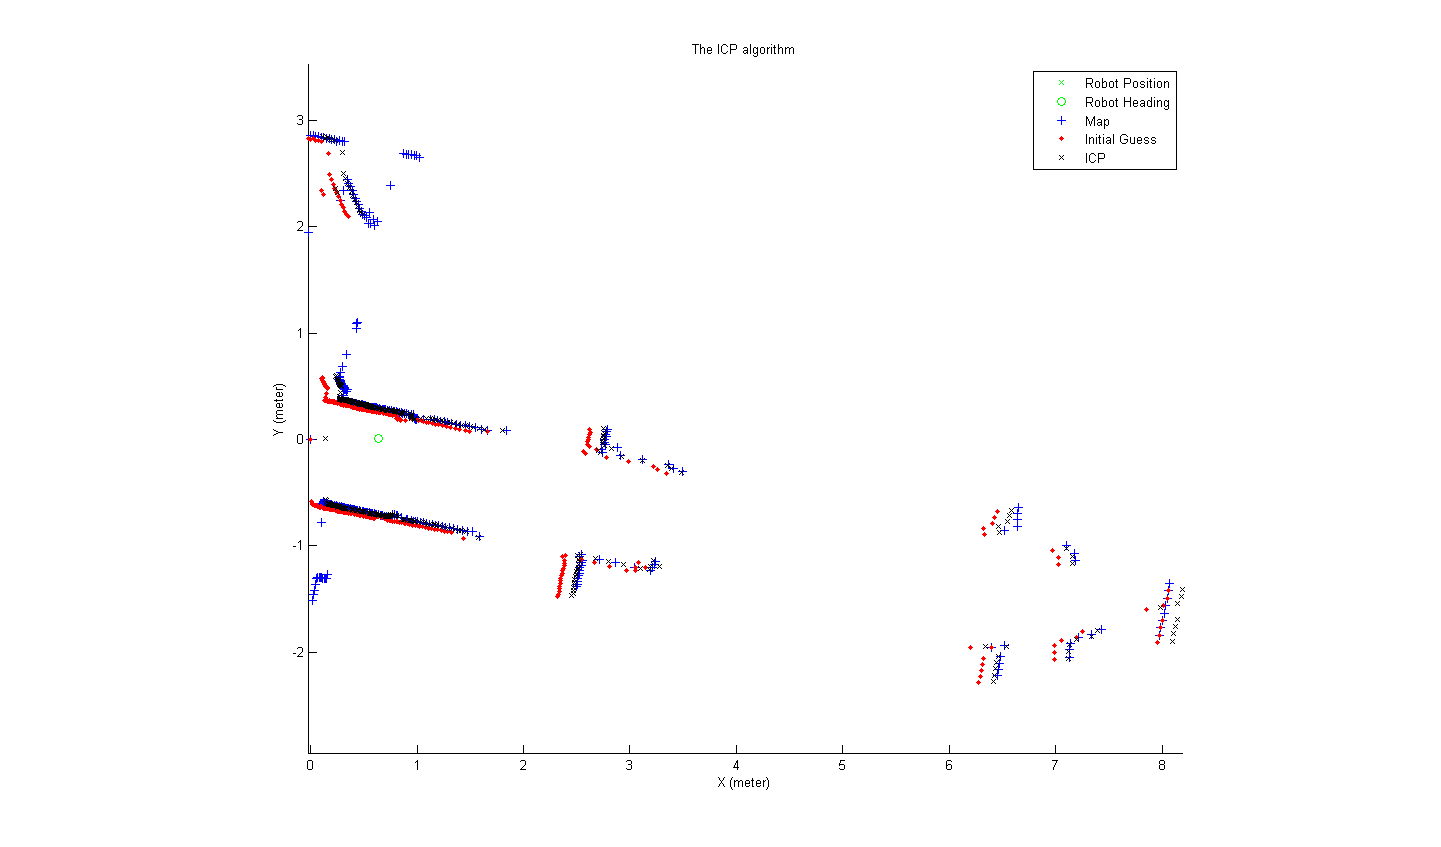
\includegraphics[scale=0.5]{q3a_1_3}\\
					\caption[\textit{RPYAxes}]{ICP estimate for maximum iterations of 40 and grid size of 0.005}
				\end{centering}
			\end{figure}
			
		\newline As can be seen, changing the grid size has little effect on the overall ICP . \newline It does, however, have an affect on the number of collision points detected. For a grid size of 0.005, 188 points collide. For 0.001, 32 points collide, and for 0.01, 252 points collide. This is expected - an increase in in the grid size means a large sample section, with a greater likelihood of multiple points landing in a grid.\newline \newline
		Checking for matching pairs reveals an interesting point - for all tested values for grid size, the number of matching points is the same - 362. Also of worthy note, despite a maximum number of iterations of 40, no more than 9 iterations are used. Changing the maximum number of iterations to 10 resulted in no changes to any of the previous tests. As such, the maximum iterative size does not need to be nearly so large.\newline \newline
		
		Looking at the generated deltaPose_bar, we can get an idea of the estimated heading of the vehicle, and by looking at deltaPose_bar_cov, we can speculate on the relationship of the system.\newline The pose was as follows:\newline \newline
		
			${deltaPose_{bar} = [0.1360,	0.0116,	 0.0004]}$ where the pattern is ${[x,y, \theta]}$
		
		\newline This Is very close to the zero position, which is to be expected seeing as this ICP algorithm has only taken a single frame. Relative movement should be little at this point.\newline
		The Pose covariance for this is as follows:\newline
		
		$$
		deltaPose_bar_cov = 1.0^-5 * 
		\begin{pmatrix}
		0.2924 & 0.0130 & -0.0099\\
		0.0130 & 0.4039 & -0.0863\\
		-0.0099  & -0.0863 & 0.0659\\
		\end{pmatrix}
		$$
		\newline
		As can be seen, the covariance matrix is extremely close to zero. This is indicative of the factors involved being completely independent, though it does not confirm this. Again, seeing as this is run from a single frame, it is not an indicator for the overall relationship - we have used far too few data points to be able to rule anything out.\newline \newline
		
		\textbf{Problems with the Algorithm}\newline
		ICPv4.m takes little into account to do with angles/rotations, mostly using x and y values. This would mean that any rotational movement in the map would be taken poorly into account, as will be evident further on.\newline \newline
				
			\pagebreak
		\subsubsection{PartB}
		\newline
		Incorporating the ICPv4.m algorithm into the laserShowACFR.m program enables us to build a real time picture of the movement of the vehicle and its perceived surroundings, relative to the actual mapped data. Observe:\newline \newline
		
		\begin{figure}[position = here]
			\begin{centering}
				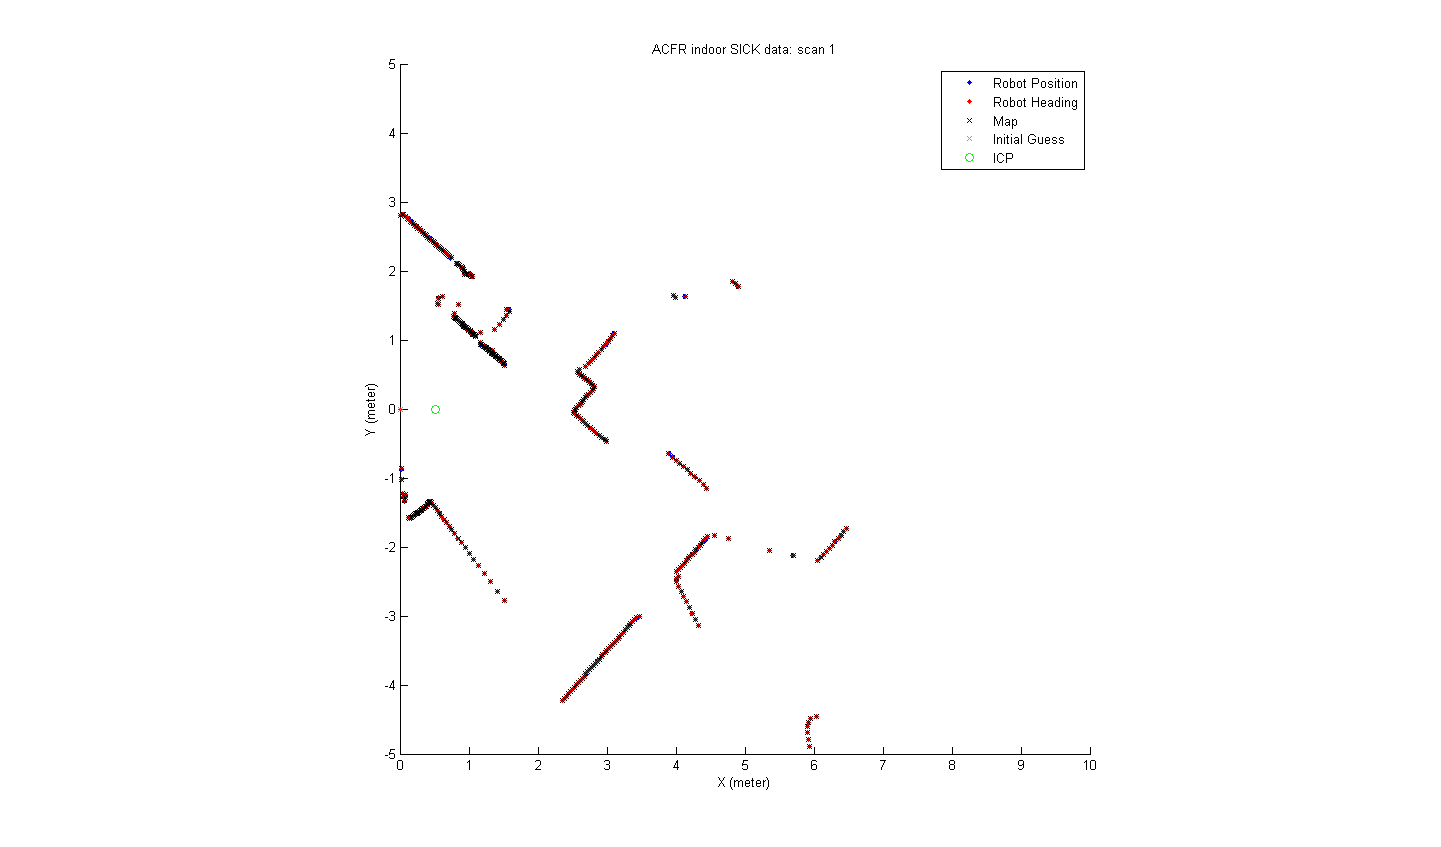
\includegraphics[scale=0.5]{q3b_scan1}\\
			\end{centering}
		\end{figure}
		\begin{figure}[position = here]
			\begin{centering}
				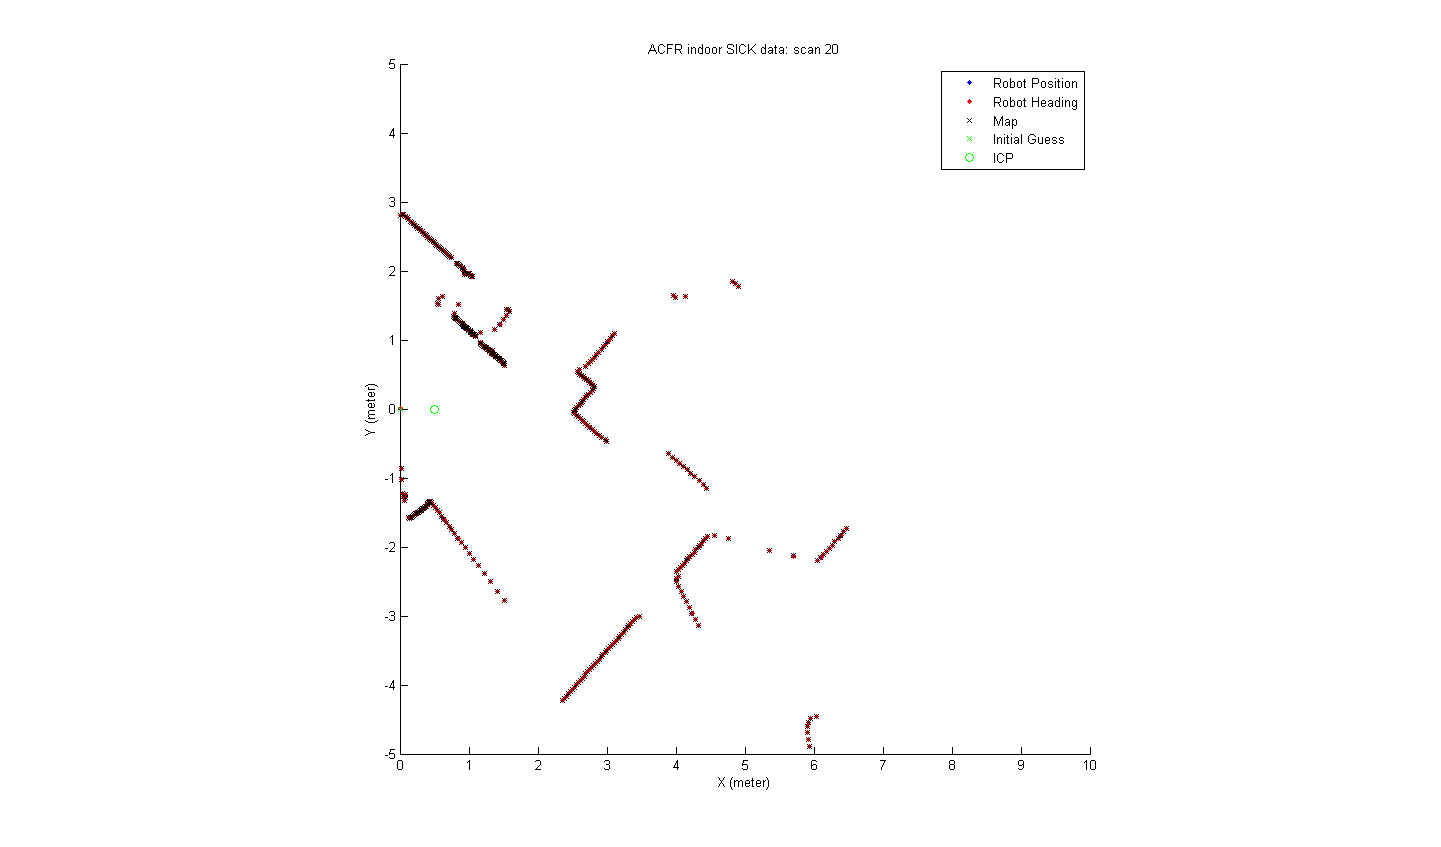
\includegraphics[scale=0.5]{q3b_scan20}\\
			\end{centering}
		\end{figure}
		\begin{figure}[position = here]
			\begin{centering}
				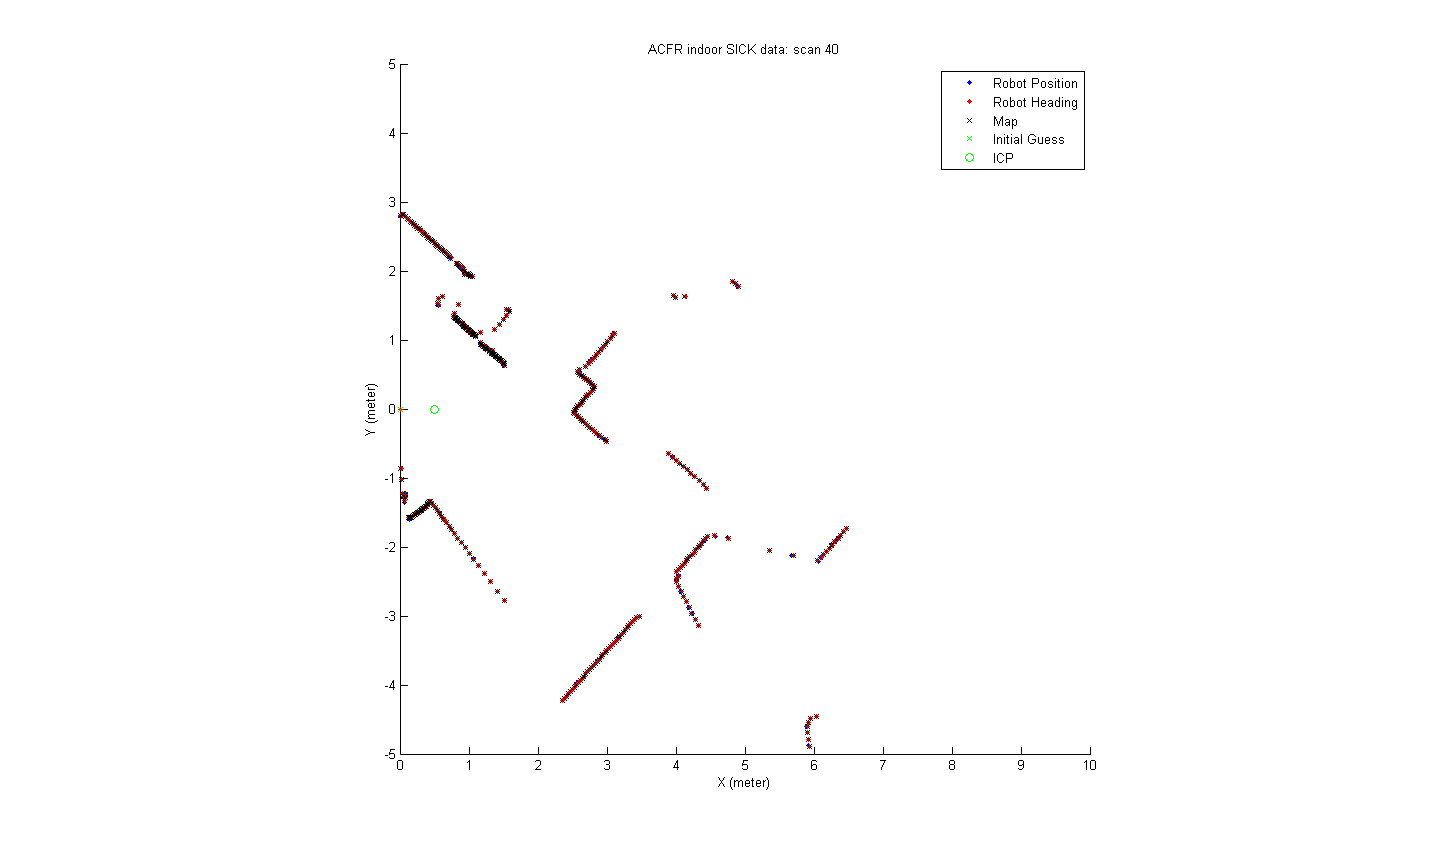
\includegraphics[scale=0.5]{q3b_scan40}\\
			\end{centering}
		\end{figure}
		\begin{figure}[position = here]
			\begin{centering}
				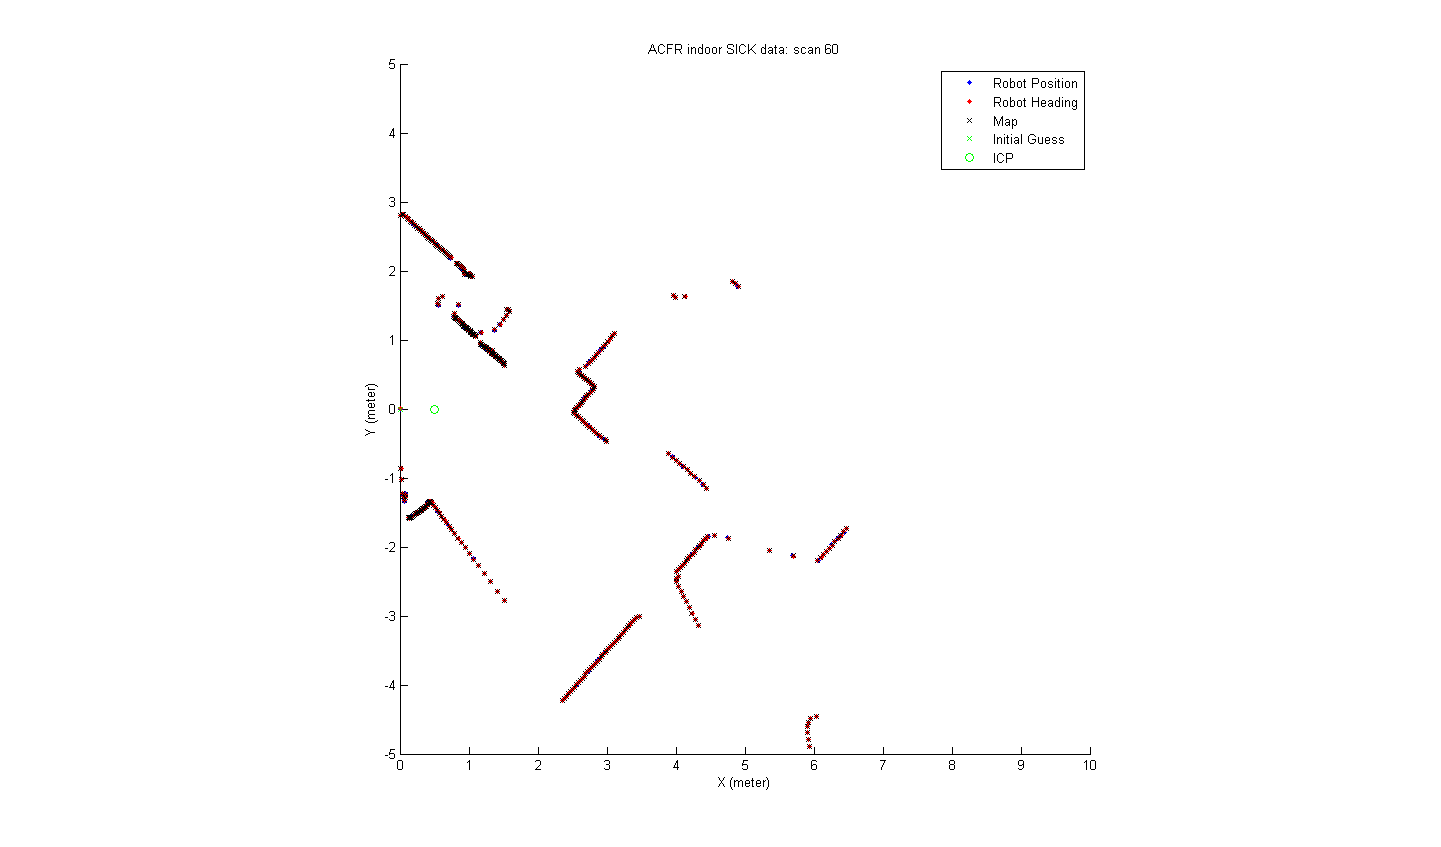
\includegraphics[scale=0.5]{q3b_scan60}\\
			\end{centering}
		\end{figure}
		\begin{figure}[position = here]
			\begin{centering}
				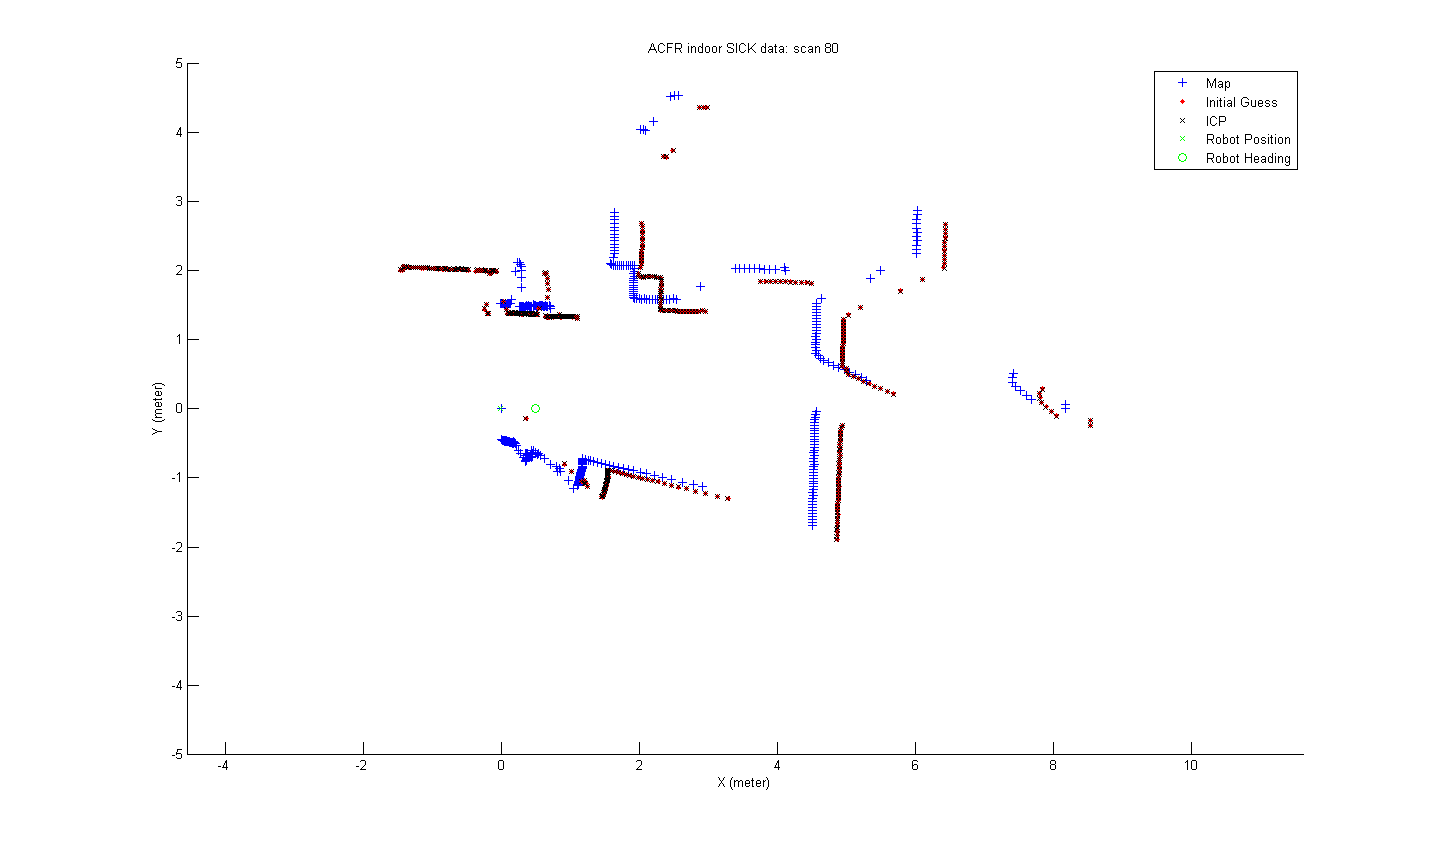
\includegraphics[scale=0.5]{q3b_scan80}\\
			\end{centering}
		\end{figure}
		\begin{figure}[position = here]
			\begin{centering}
				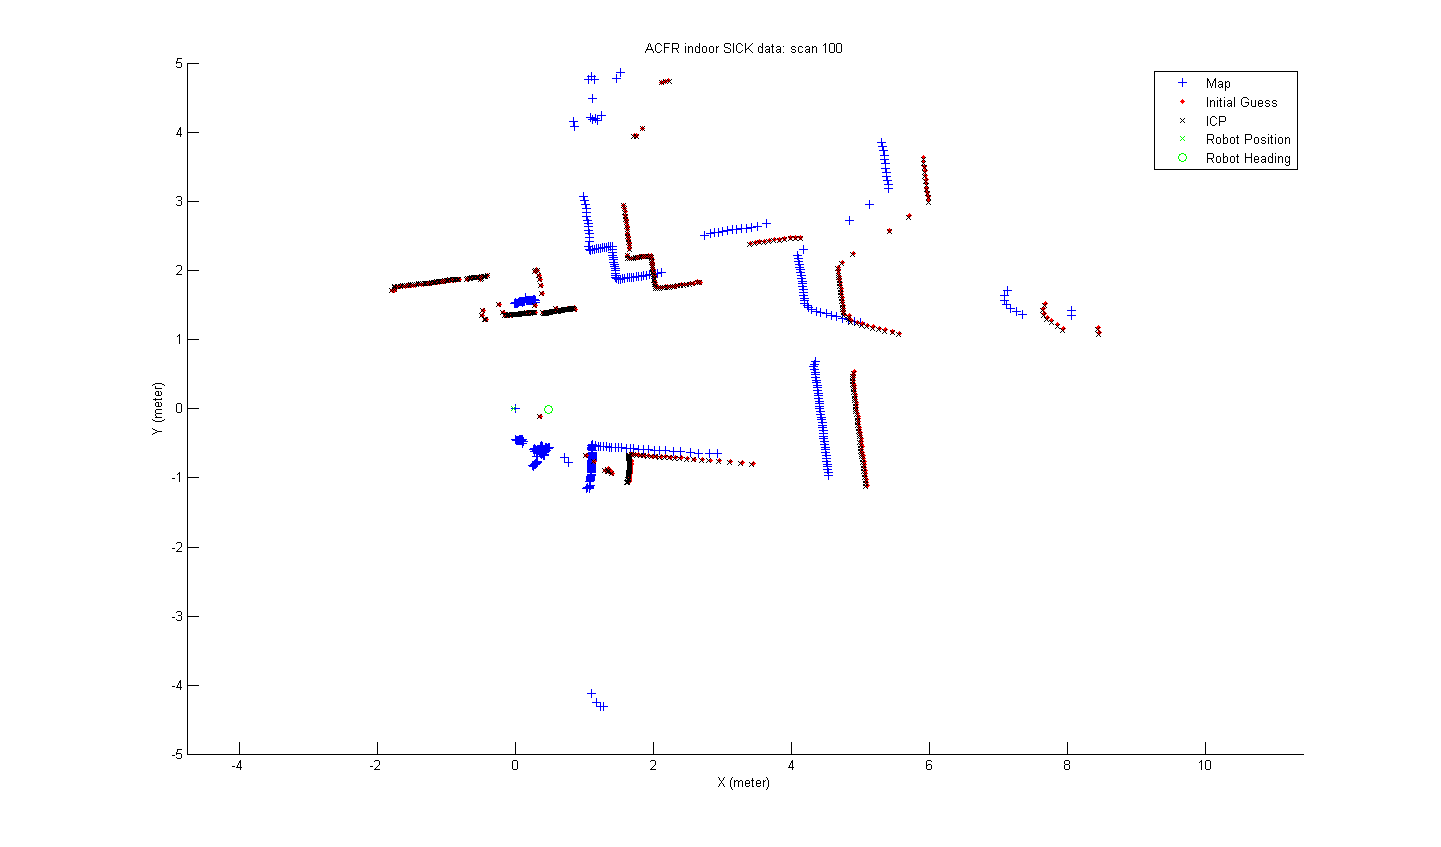
\includegraphics[scale=0.5]{q3b_scan100}\\
			\end{centering}
		\end{figure}
		\begin{figure}[position = here]
			\begin{centering}
				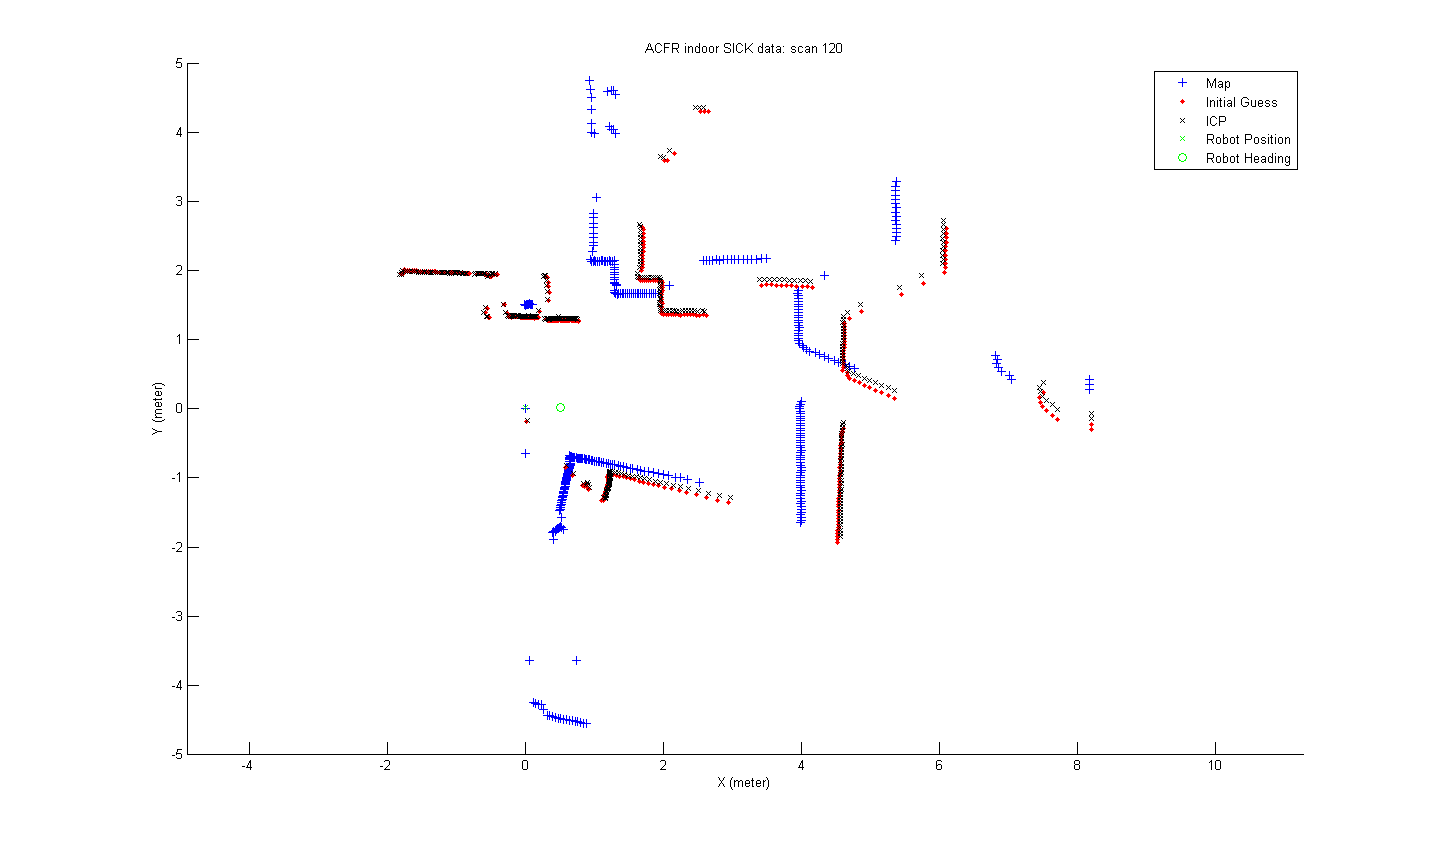
\includegraphics[scale=0.5]{q3b_scan120}\\
			\end{centering}
		\end{figure}
		\begin{figure}[position = here]
			\begin{centering}
				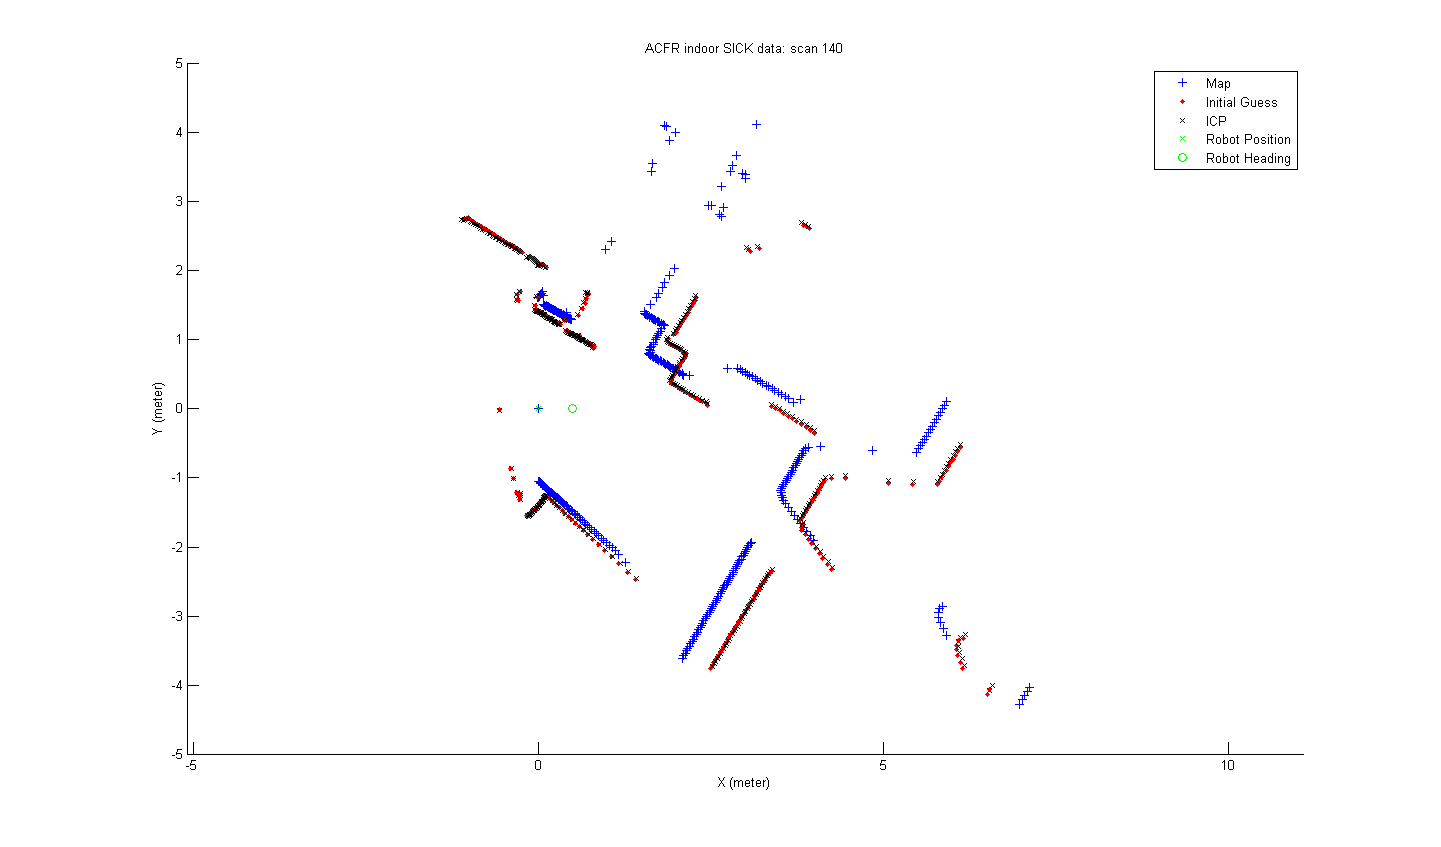
\includegraphics[scale=0.5]{q3b_scan140}\\
			\end{centering}
		\end{figure}
		\begin{figure}[position = here]
			\begin{centering}
				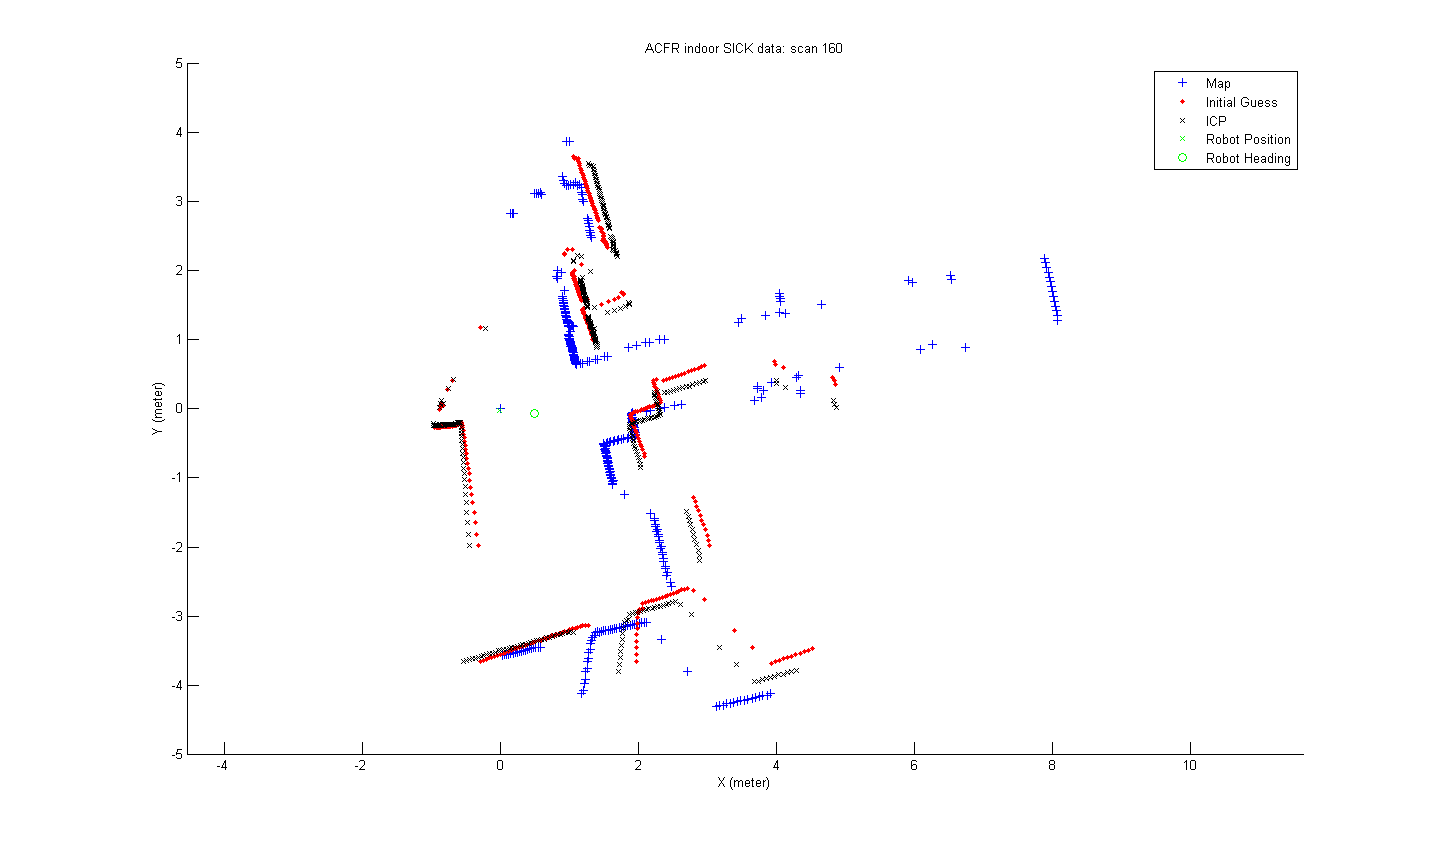
\includegraphics[scale=0.5]{q3b_scan160}\\
			\end{centering}
		\end{figure}
		\begin{figure}[position = here]
			\begin{centering}
				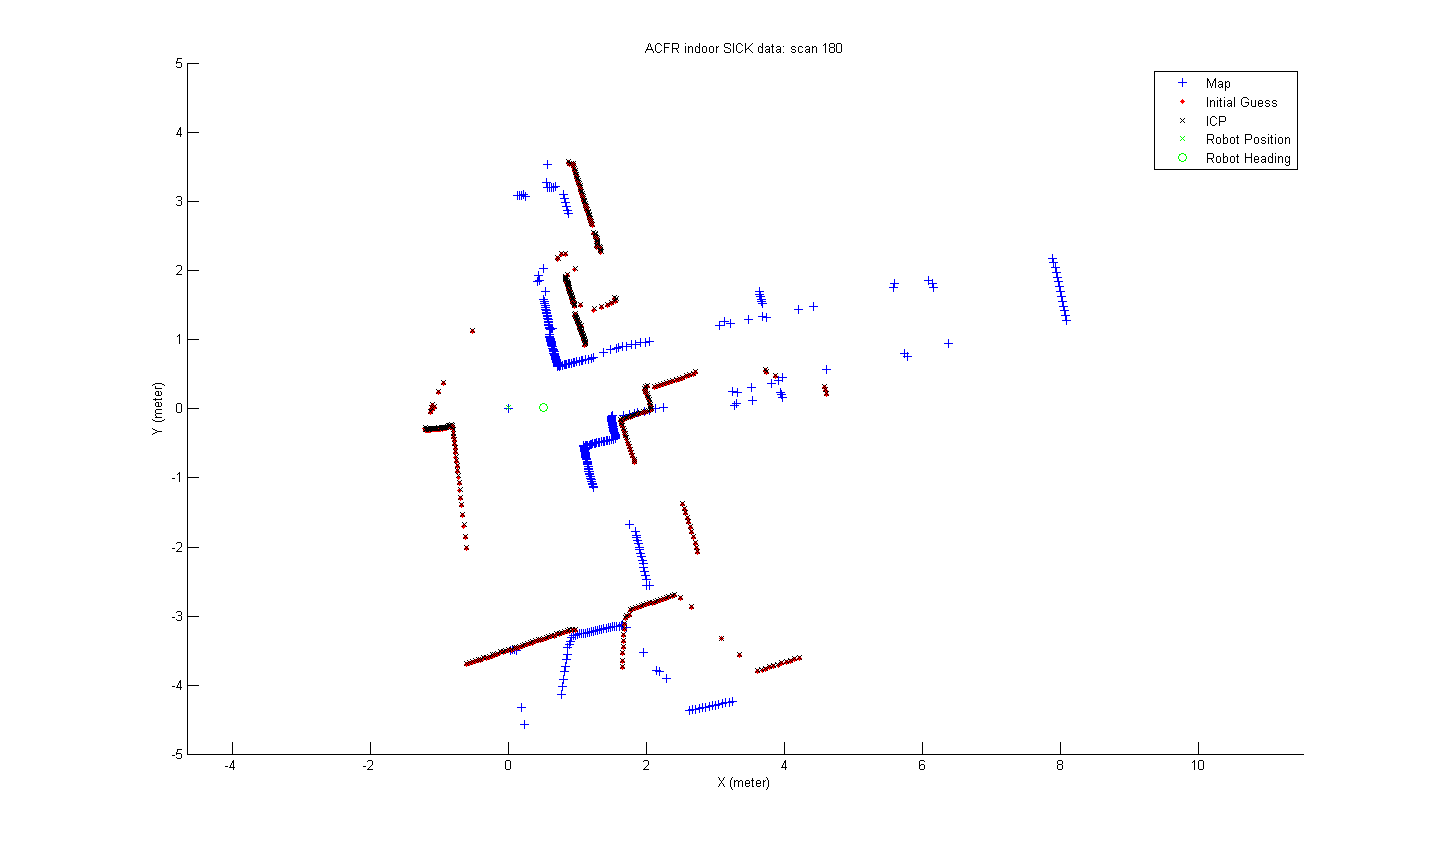
\includegraphics[scale=0.5]{q3b_scan180}\\
			\end{centering}
		\end{figure}
		\begin{figure}[position = here]
			\begin{centering}
				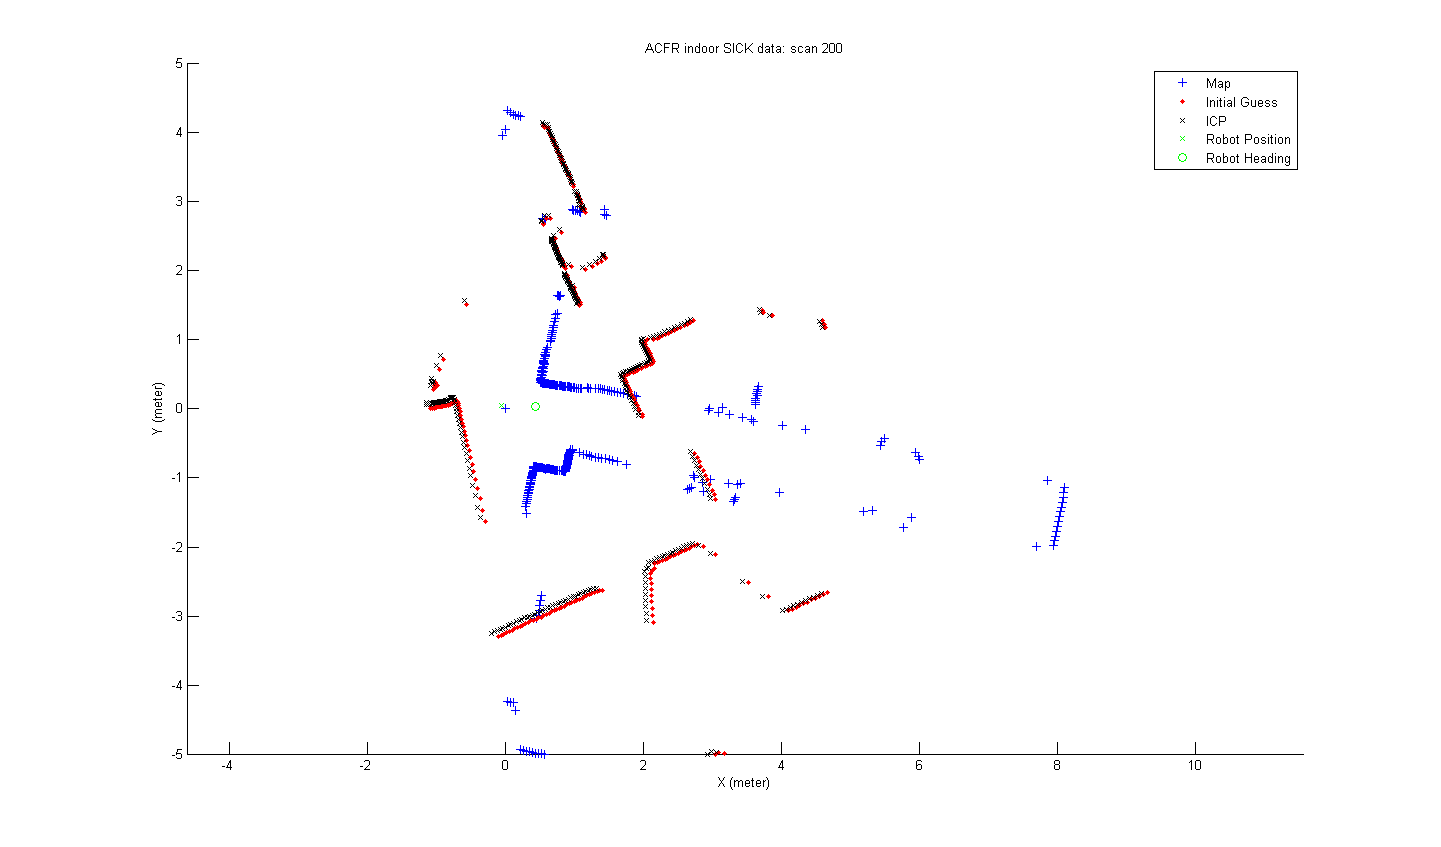
\includegraphics[scale=0.5]{q3b_scan200}\\
			\end{centering}
		\end{figure}
		\begin{figure}[position = here]
			\begin{centering}
				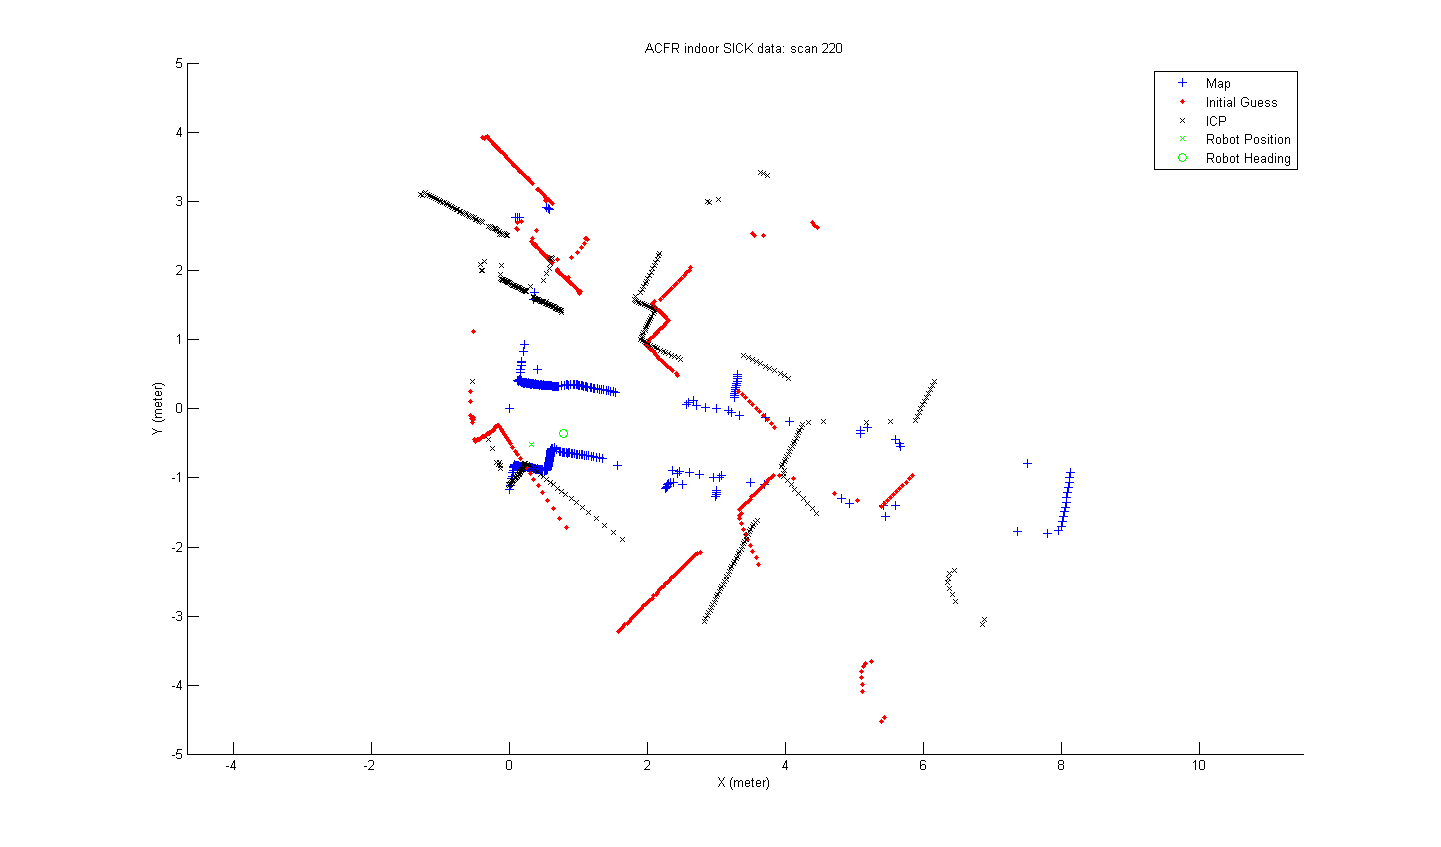
\includegraphics[scale=0.5]{q3b_scan220}\\
			\end{centering}
		\end{figure}
		\begin{figure}[position = here]
			\begin{centering}
				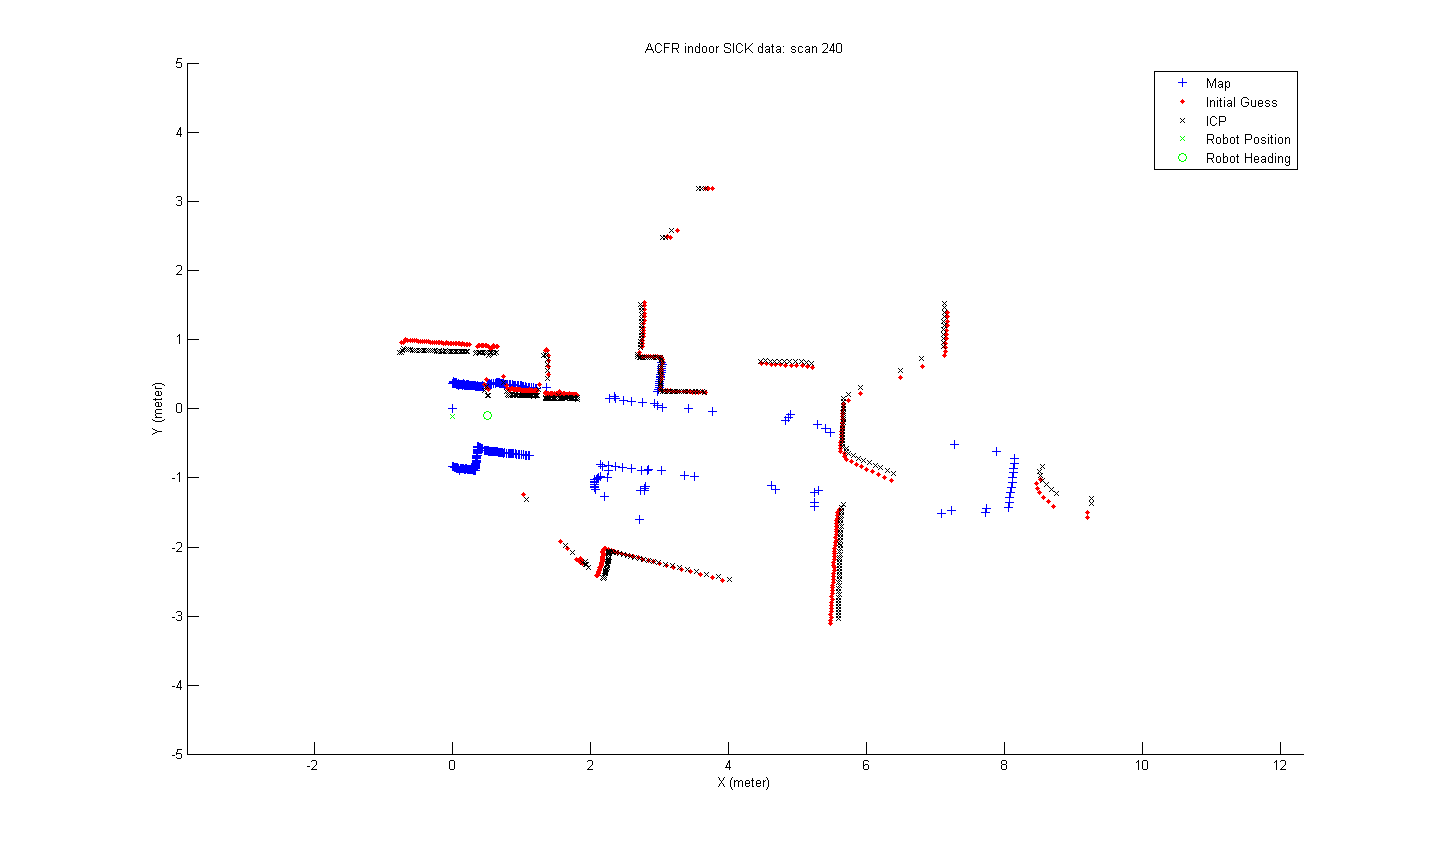
\includegraphics[scale=0.5]{q3b_scan240}\\
			\end{centering}
		\end{figure}
		\begin{figure}[position = here]
			\begin{centering}
				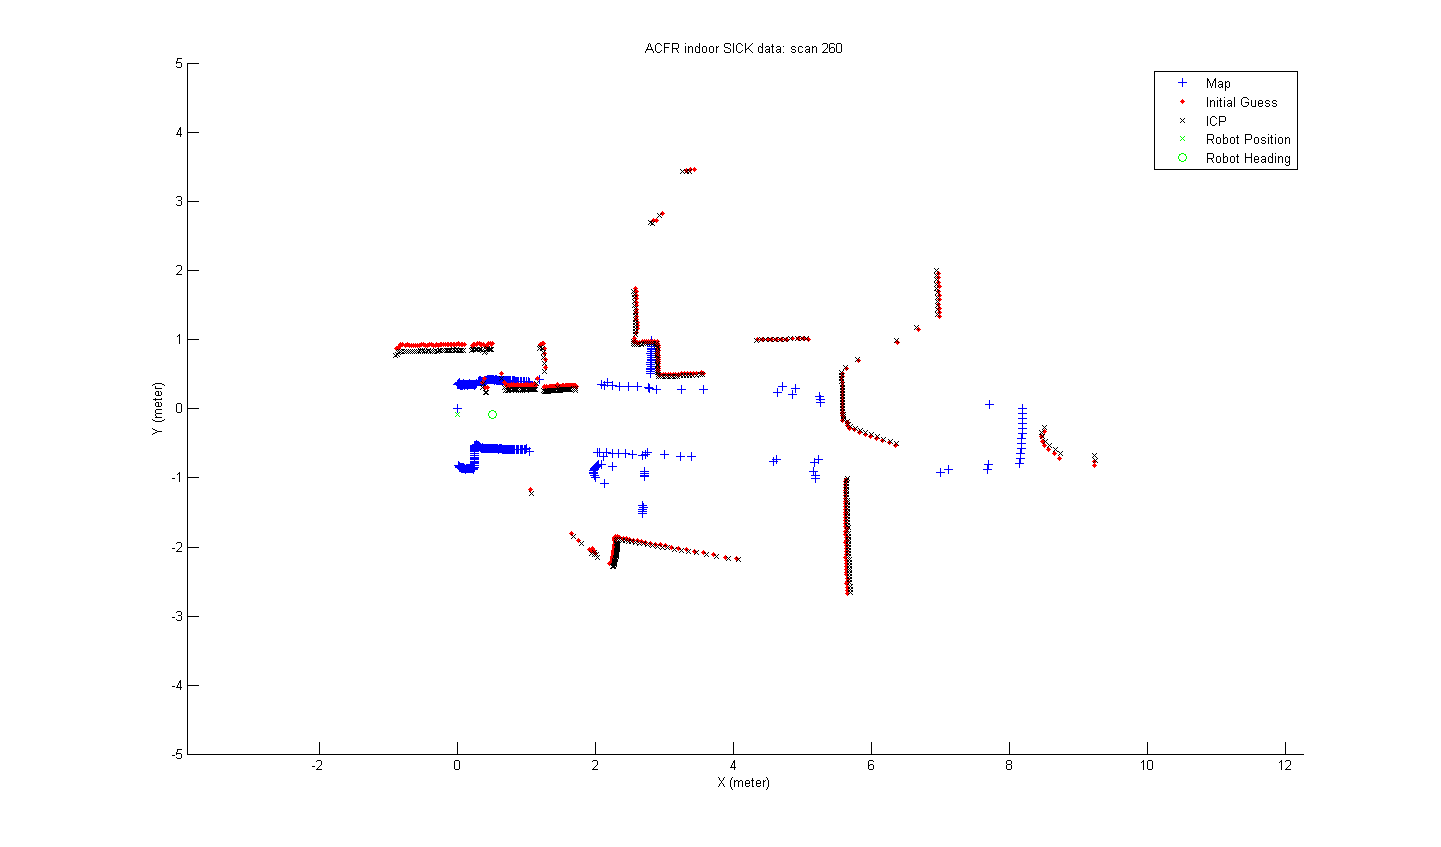
\includegraphics[scale=0.5]{q3b_scan260}\\
			\end{centering}
		\end{figure}
		\begin{figure}[position = here]
			\begin{centering}
				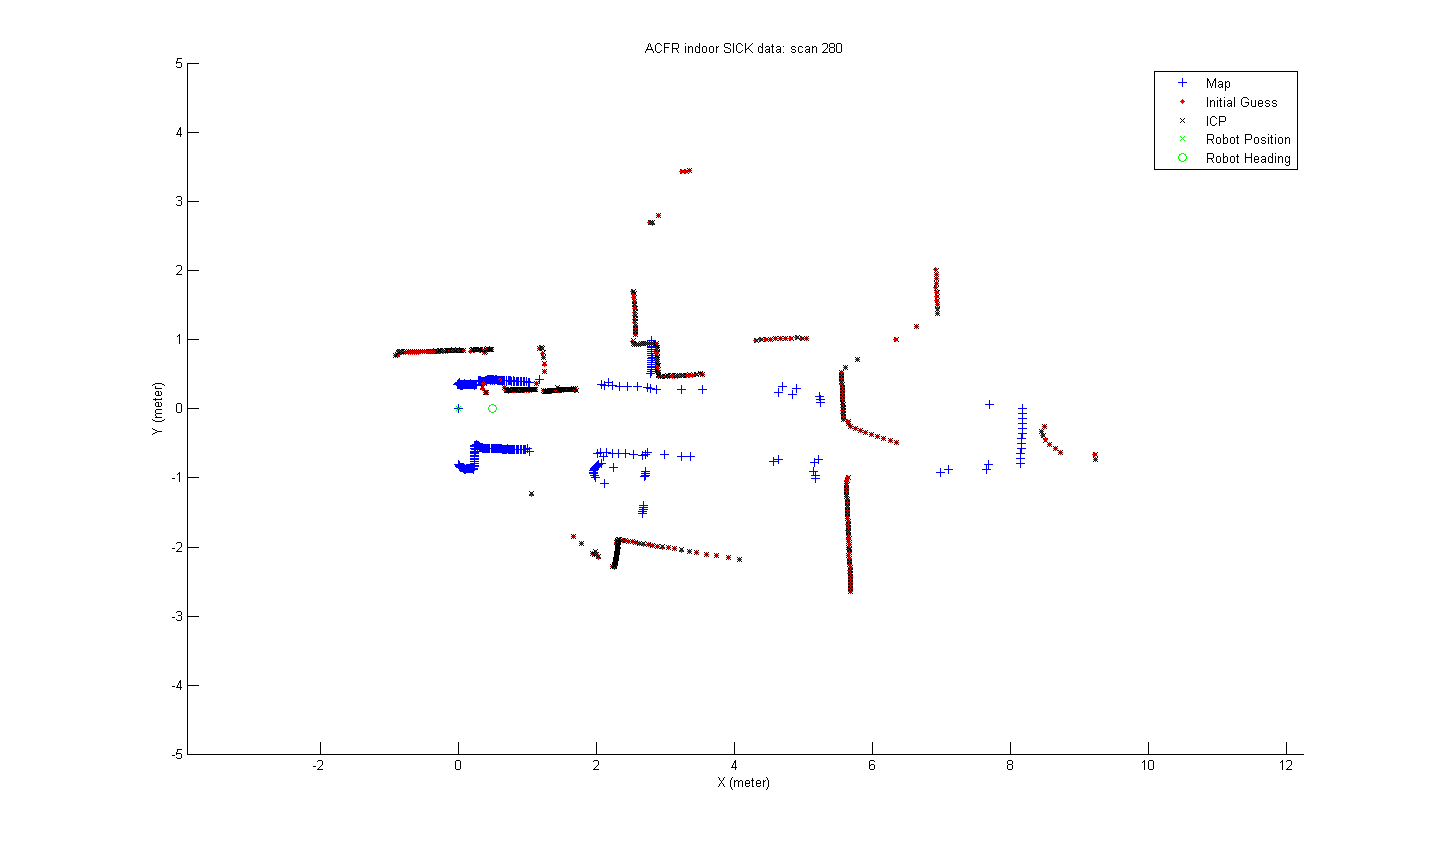
\includegraphics[scale=0.5]{q3b_scan280}\\
			\end{centering}
		\end{figure}
		\begin{figure}[position = here]
			\begin{centering}
				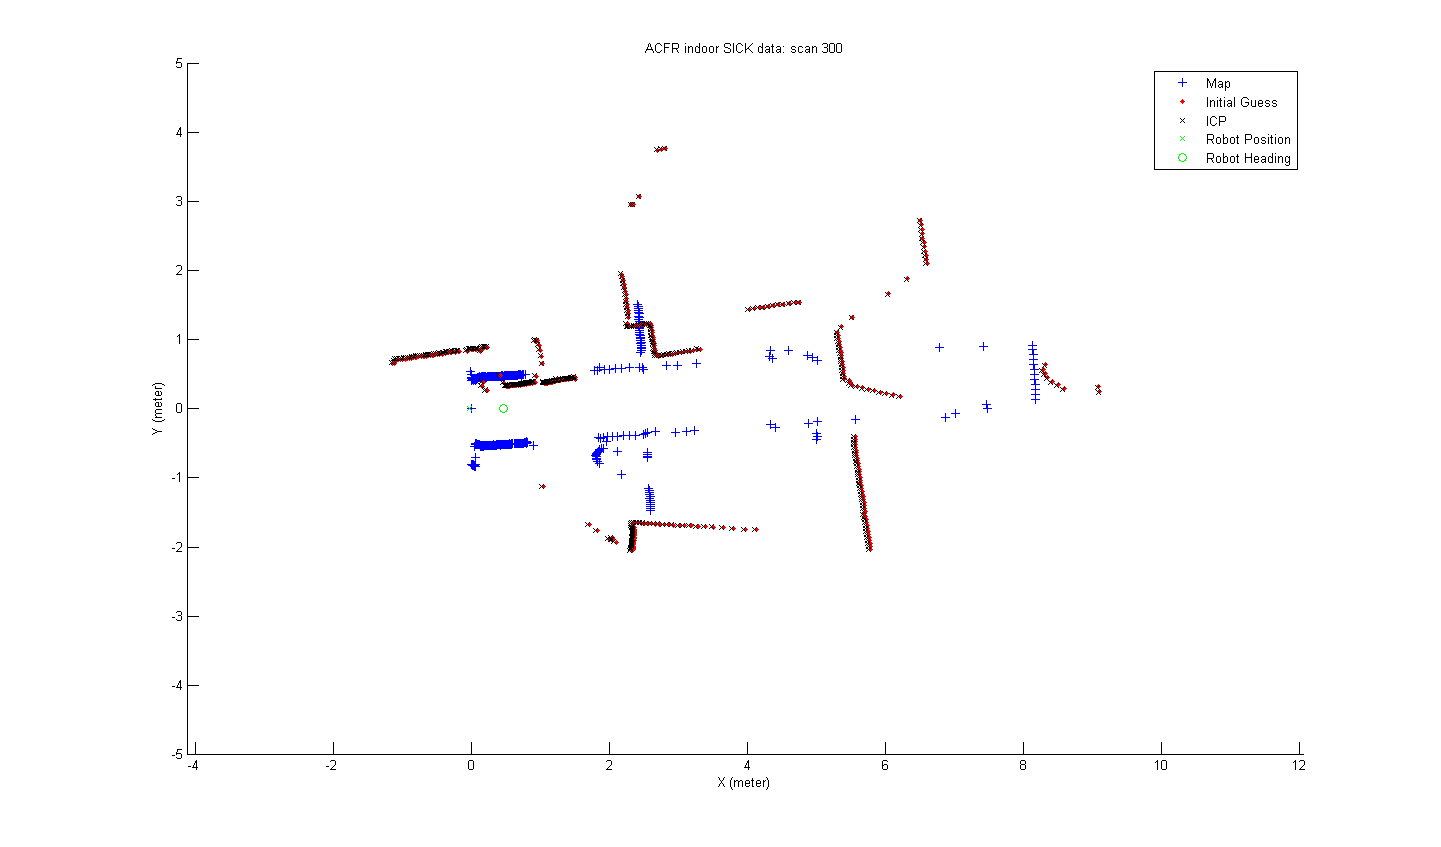
\includegraphics[scale=0.5]{q3b_scan300}\\
			\end{centering}
		\end{figure}
		\newline
		\newline
		\pagebreak
		As can be seen, the ICP initially tracks the map data rather well, and the vehicle remains roughly alligned with the direction of motion. Around scan 200 however, everything begins to break down. At this point, the ICP has started lagging behind, and when the vehicle suddenly rotates it is unable to keep up. The closest points now no longer correspond to the original positions, and the ICP map becomes distorted, aligining with a new set of map data points. By scan 300 the alignment is well an truly distorted, with the ICP data almost backwards on the map data. The scans remain relatively unchanged for the next thousand frames, which have not been shown here. The vehicle, suprisingly, appears to be orientated correctly. This is probably a fluke.\newline \newline
		Considering that at some points in the scans the ICP vehicle position placed it in or beyond the walls, this would not be a particularly effect method of guidance.\newline \newline
		Note, however, that though there was always some offset between the ICP map and the real map, this offset was almost constant. The greatest offset would occur during rotations, which the ICP was able to follow initially. However, these first few rotations where slow, enabling the ICP algorithm to keep up. Around frame 200, the first rapid rotation took place, and the ICP finally failed to keep up, recognising new points as the closest and pairing with them.\newline
		As mentioned above, this is because the ICP algorithm fails to take this rotational element into account. However, the given algorithm would still be acceptable under the correct circumstances. With either far more data points taken per seconds, enabling the ICP to 'linearise' the rotations, would enable it to handle sudden rapid rotations. Alternatively, the vehicle could be drastically slowed down, resulting in more data points through the rotation, again enabling some degree of linearity.
		\newline
		

		
	\pagebreak

	\subsection*{Code Listing}
	See Appendix A [3] for all code used.
